% Součást skript na Datové struktury. Viz main.tex
% přepsal Vladimír Kotal, 2003


% nasleduje prednaska z 19.3.2003, přepsal Vladimír Kotal

\markright{$ $Id$ $}

\chapter{Samoopravující se struktury}

Upravující algoritmy pracují na seznamech, mohou přemístit prvek, 
který je argumentem operace. (pokud zůstává v seznamu) 
Čas na vyhledání - to je pozice hledaného prvku. Pokud není v seznamu, je
to délka seznamu + 1.
\par

Pokud byl prvek na $i$-tém místě a přesune se na $j$-té, tak je-li\\
  $j < i$, provedou $i-j$ volných výměn\\
  $j > i$, provedou $j-i$ placených výměn
\par

Volné výměny se nezapočítávají do složitosti.
Pokud x není v seznamu při operaci INSERT(x), tak předpokládejme, že je na
1. pozici po ukončení seznamu.


% --------------------------------------------------------------------------
\section{Seznamy}

{\mnote XXX operace nad obycejne seznamy jsou velmi jednoduche. Všechny
musí lineárně projít celý seznam než provedou danou operaci.}

MEMBER
INSERT
DELETE


% MFR -----------------------------------------------------------------------

\subsection{Algoritmus MFR (Move Front Rule)}
\mnote{přednáška z 18.3.2003}

{\bf Pravidlo MFR}: Při operaci MEMBER(x) je $x$ v seznamu nebo při 
operaci INSERT($x$) bude $x$ po skončení operace na 1. místě seznamu.

\begin{theorem}
\label{theor:samoop.MFRtime}
Mějme posloupnost $P$ operací MEMBER, INSERT a DELETE a mějme dva
prosté seznamy $S1$, $S2$ množiny $S$. \\
Pak pro každý upravující algoritmus $A$ platí:\\
Když MFR provede $P$ na seznam $S1$ a A provede $P$ na seznam $S2,$ 
tak platí:
\par

Označíme:
\begin{itemize}
\item $s$ = čas na vyhledání A
\item $p$ = počet placených výměn A
\item $f$ = počet volných výměn A
\end{itemize}

Pak čas MFR $\leq$ 
\(
  \begin{cases}
  s + p - f - |P| 
  	& \text{když } S1 = S2 \\

  s+ p - f - |P| + \binom{|S|}{2}
  	& \text{když } S1 \neq S2 
 \end{cases}
\)

\end{theorem}

\begin{defn}
Nechť $S1$, $S2$ jsou dva prosté seznamy množiny $S$, pak $bal(S1,S2)$ je
počet neuspořádaných dvojic $\{x,y\}$, $x \neq y$, $x,y \in S$ takových že 
$x$ je před $y$ v $S1$ a $y$ je před $x$ v $S2$.
\end{defn}

\begin{pozn}
Platí \\
\begin{itemize}
\item $bal(S1,S2) = 0 \Leftrightarrow S1 = S2$ (prvky jsou ve stejném
	pořadí $\Leftrightarrow$ seznamy jsou stejné)
\item $bal(S1,S2) \leq \binom{|S|}{2}$ (všechny dvojice jsou přeházené)
\end{itemize}
\end{pozn}

\begin{proof}[Důkaz věty \ref{theor:samoop.MFRtime}] 
\mnote{tento dukaz je nejaky podivny}
Přes amortizovanou složitost A. \\
Předpokládejme, že A i MFR mají provést operaci O.\\
A ... provádí na seznam $S_A$, výsledek bude $S_A'$ \\
MFR .. provádí O na seznam $S_{MFR}$, výsledek bude $S_{MFR}'$\\
amortizovaná složitost operace O bude: 
$$
= \text{čas MFR pro operaci } O + bal(S_A', S_{MFR}') 
  - bal(S_A, S_{MFR})
$$
Balance $bal$ je definována vzhledem k algoritmu A.
\par

Ukážeme, že amortizovaná složitost $O$ pro MFR 
$$
\leq 2*\text{čas na vyhledání A} +
\text{počet placených výměn A} - \text{počet volných výměn A} - 1
$$

$$
{\rm S_A}\stackrel{\text{vyhledání}}{\rightarrow} S_A''
\stackrel{\text{výměny}}{\rightarrow} S_A'
$$
$$
{\rm S_{MFR}} \rightarrow S_{MFR}' \rightarrow S_{MFR}'
% XXX carkovana sipka
$$
\par

kde po operaci \\

\begin{tabular}{|l|l|}
\hline
DELETE(x) & $S_A''$ = $S_A'$\\
MEMBER(x) & $S_A''$ = $S_A$\\
INSERT(x) & $x$ je v seznamu , $S_A''$ = $S_A$\\
  	  & $x$ není v seznamu, $S_A''$ vznikne z $S_A'$ přidáním $x$ za
		poslední prvek seznamu\\
\hline
\end{tabular}

\hspace{8mm}

% \(
% \begin{cases}
%  x\ je\ v\ seznamu , S_A'' = S_A\\
%  x\ není\ v\ seznamu, S_A''\ vznikne\ z\ S_A'\ přidáním\ x za poslední prvek seznamu
% \end{cases}
% \)


Podstatné je, že seznamy jsou nad stejnou množinou.
\par

Amort. složitost první části $\leq 2*\text{čas na vyhledání pro } A - 1$ \\
Amort. složitost druhé části $= \text{počet placených výměn A} - 
\text{počet volných výměn A}$
\par

% jak donutit itemize aby cislovalo pomoci i, ii, iii, ... ?
\begin{itemize}
\item[(i)]
Předpokládejme, že x není v seznamu a délka seznamů je $n$.
Čas MFR je $n+1$ , čas na vyhledání pro algoritmus je $n+1$
operace MEMBER(x) a DELETE(x) $S_A''$ = $S_{MFR}'$
a tedy amort. slož. MFR = čas operace = $n+1 \leq 2(n+1) - 1$ \\
$n+1$ je čas na vyhledání pro $A - 1$ \\
$S_A''$ vznikne z $S_A$ přidáním $x$ za posl. prvek $S_A$ \\
$S_{MFR}'$ vznikne z $S_{MFR}$ přidáním $x$ na zač. seznamu
tedy 
$$
bal(S_A'', S_{MFR}') - bal(S_A, S_{MFR}) = n
$$
Amort. slož. operace MFR 
$= n+1 + n=2n + 1=2(n+1) - 1 = 2*\text{čas na vyhledání A} - 1$

\item[(ii)] $x$ je v seznamu. Předpokládejme, že $x$ je na $i$-tém místě v
seznamu $S_A$ na $j$-tém místě v seznamu $S_{MFR}$
Čas operace pro MFR je $j$, čas na vyhledání pro $A$ je $i$.
Označme $k$ počet $y$ v seznamu takových, že $y$ je v $S_A$ za $x$, v
$S_{MFR}$ před $x$.
\par
Pak $i+k \geq j$ ($i+k \geq i-k+j$)
amort. slož. pro MFR 
$= j + bal(S_A'', S_{MFR}') - bal(S_A, S_{MFR})$
\par

\begin{itemize}
  \item DELETE(x)\\
  $bal(S_A'', S_{MFR}') - bal(S_A, S_{MFR}) \leq -k$ \\
  amort. slož. $\leq j - k \leq 2i - 1 = 2*\text{čas na vyhledání A - 1}$
  
  \item MEMBER(x), INSERT(x) \\
  $bal(S_A'', S_{MFR}') - bal(S_A, S_{MFR}) \leq -k + i-1$
  (nějaké dvojice mohly přibýt) \\
  amort. slož. operace MFR 
  $\leq j-k+i-1 \leq i+i-1 = 2i - 1 = 2*\text{čas na vyhledání A} - 1$
\end{itemize}
\end{itemize}


\subsubsection{Amort. složitost}

\begin{enumerate}
\item fáze operace $\leq 2*\text{čas na vyhledání A} - 1$
\item fáze operace 
	$= \text{počet placených výměn A} - 
	\text{počet volných výměn A}$
\end{enumerate}

Při placené výměně si v seznamu $S_A''$ vymění $x$ místo $z$ za $x$, tedy
dvojice $\{x,z\}$ přibude při počítání 
$bal(S_A', S_{MFR}') - bal(S_A'', S_{MFR}')$ \\
(v $S_{MFR}$ je x první)
\par
Při volné výměně se v seznamu $S_A''$ vymění $x$ místo s prvkem $u$ před
$x$, tedy dvojice $\{x,u\}$ se vynechá při počítání $bal$.
Amort. slož. MFR $\leq 2*\text{čas na vyhledání A} +
\text{počet placených výměn A} - \text{počet volných výměn A} - 1$
\par

Tedy platí: \\
čas posloupnosti P pro MFR 
$\leq \text{odhad amort. složitosti} + bal(S_1, S_2) = 
2*\text{čas na vyhledání v P algoritmem A} + 
\text{počet placených výměn A při P} - 
\text{počet volných výměn A při P} - |P| + bal(S_1, S_2)$

\mnote{$|P|$ ... za každou operaci je -1}

\begin{itemize}
\item když $S_1$ = $S_2$ pak $bal(S_1, S_2)=0$ a platí a)
\item když $S_1 \neq S_2$ pak $bal(S_1, S_2) \leq \binom{|S|}{2}$ a
platí b)
\end{itemize}
\end{proof}

\mnote{temporary solution by T.Matoušek}

\subsubsection{Očekávaná složitost MFR}

% XXX kdyz dukaz, tak by tady melo byt nejake tvrzeni

\begin{proof}
$E_{MFR} = \sum l_i p_i$
kde $l_i$ je očekávaná vzdálenost $x_i$ od začátku seznamu a $p_i$ je
pravděpodobnost, že se budeme ptát na $x_i$.
\par
$$
l_i = 1 + E(\sum\limits_{j=1}^n Y_{ij})
$$

Jednička je tam za prvek $x_i$, kde $Y_{ij}$ je náhodná proměnná s 
alternativním rozdělením s pravděpodobností $p_{ij}$ a
říká, jestli je prvek $x_j$ před $x_i$.
\par
Průměr součtu je součet průměrů, takže platí: \\
$$
l_i = 1 + \sum\limits_{j=1}^n EY_{ij}
$$

Dále víme, že $EY_{ij} = p_{ij}$, nebo-li
$$
l_i = 1 + \sum\limits_{j=1}^n p_{ij}
$$
\par

Zbývá tedy spočítat $p_{ij}$ : \\

\begin{equation}
\begin{split}
p_{ij} & = p(\text{``} x_j \text{ bude před } x_i \text{``}) \\
& = p(\text{poslední MEMBER, který byl na }x_i \text{ nebo } x_j\text{,}
\text{byl na } x_j \text{``}) \\
& = p(\text{``poslední zavolání MEMBER bylo na } x_j \text{``} | 
\text{``poslední zavolání MEMBER bylo na } x_i \text{ nebo } x_j \text{``}) \\
& \stackrel{*}{=} p(\text{``zavolání MEMBER na } x_j \text{``} | 
\text{``zavolání MEMBER na } x_i \text{ nebo } x_j \text{``}) \\
& = \frac{p_j}{p_i + p_j}
\end{split}
\end{equation}
\mnote{* - každé volání MEMBER na daný prvek je stejne pravděpodobné}

Když to dáme dohromady:
$$
E_{MFR} = \sum l_i p_i = \sum [1 + \sum\limits_{j=1}^n \frac{p_j}{p_i +
p_j}] p_i = 1 + \sum\limits_{i, j = 1}^{n} {p_i p_j}{p_i + p_j}
$$
\end{proof}

\begin{pozn}
S tímto jsme se setkali při EISCH. \\
Je to důvod, proč je EISCH lepší než LISCH, VICH lepší než LICH.
\end{pozn}

% TR -----------------------------------------------------------------------

\subsection{Algoritmus TR (Transposition Rule)}

Když je $x$ při operaci MEMBER($x$) a INSERT($x$) na $i$-tém místě, 
tak ho dá přísl. operace na ($i-1$)-ní místo.
\par
Pokud při INSERT($x$) není $x$ v seznamu, INSERT umístí $x$ na předposlední 
místo.
\par

\begin{pozn}
Lze najít posloupnost příkazů $P$ lib. délky, že MFR vyžaduje čas $(|P|)$ a
TR vyžaduje čas $(|P|^2)$. Na druhou stranu očekávaný čas TR $\leq$
očekávaný čas MFR.
\end{pozn}


Chceme spočítat očekávaný čas MFR pro posloupnosti $P$ aplikované na
seznam $S$,
kde $P$ obsahuje jen operace MEMBER($x$) pro $x \in S$. 
\par
Předpokládejme, že $S={1,2, ... , n}$ a $\beta_1$ = pravděpodobnost operace
MEMBER(x) pro $x \in S$.
$S = \{1,2,3\}$ ... stavy Markovova řetězce jsou všechny permutace $S$
pravděpodobnost přechodu je pst. operace převádějící jeden stav do
druhého.
\par

\begin{figure}[!htb]
\centering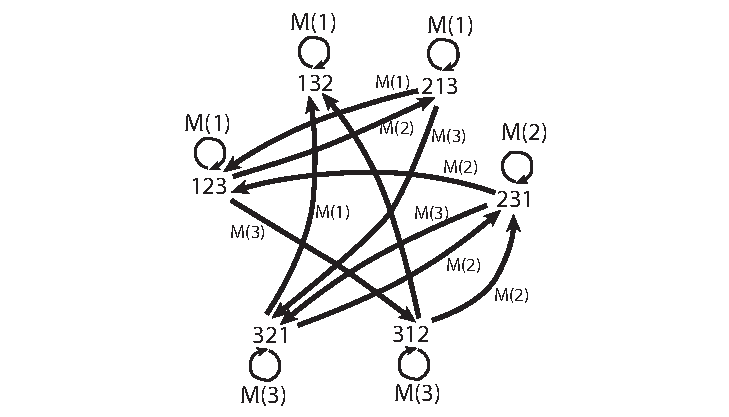
\includegraphics{pics/tr-markov}
\caption{Přechody mezi stavy}
\label{tr-markov}
\end{figure}


Tyto Markovovy řetězce jsou nerozložitelné a aperiodické a to znamená, že
existují asymptot. pravděpodobnosti, tj. pro seznam $\Pi$ je dána
pravděpodobnost ${\kappa}_{\Pi}$, že po provedení náhodné posloupnosti $P$ s
daným rozložením operací skončíme u seznamu $\Pi$.
\par

Pak očekávaný čas je $\sum_{\Pi}{\kappa}_{\Pi}\sum_{i}{\beta}_i\Pi(i)$, 
$\Pi(i)$ je pozice $i$ v seznamu $\Pi$.
\par
$p_1 = \sum_{\Pi}{\kappa}_{\Pi}\Pi(i)$ ... očekávaná pozice prvku $i$
\par
$\delta(j,i)$ = asmyptot. pst., že prvek $j$ je před $i$, pak platí \\
$$
\delta(j,i) = \sum\{\kappa_\Pi , \Pi\ seznam, \Pi(j) < \Pi(i)\}
$$

pak 
\begin{equation}
\begin{split}
p_i & = \sum_{\Pi}\kappa_\Pi\Pi(i) \\
& = \sum_{\Pi}\kappa_\Pi(1 + |{j, \Pi(j) < \Pi(i)|} \\
& = 1 + \sum{j,\Pi}\{\kappa_\Pi, \Pi(j) < \Pi(i)\} \\
& = 1 + \sum_{j}\delta(j,i) (1)
\end{split}
\end{equation}

Zkusíme $\delta(j,i)$ spočítat jiným způsobem: \\
Idea: jak se může stát, že ve výsledném seznamu je $j$ před $i$ ?
V posloupnosti $P$ existovala operace MEMBER($x$) a po ní se už nevyskytovala
operace MEMBER($i$) ani MEMBER($j$).
\par

Jaká je pravděpodobnost tohoto jevu ?
\begin{multline}
\beta_j\sum_{k=0}^{\infty}[1 - (\beta_i - \beta_j)]^k 
= \beta_j \frac{1}{1-(1-(\beta_i+\beta_j)} 
= \frac{\beta_j}{\beta_j+\beta_i} \stackrel{(1)}{=} 
1 + \sum_{\substack{j,i\\j \ne i}} \frac{\beta_j}{\beta_j+\beta_i}
\end{multline}

Očekávaný čas operace \mnote{jake operace ? XXX} je 
$$
\sum_{i} \beta_i p_i 
= \sum_{\substack{j,i\\j \ne i}} \frac{\beta_i\beta_j}{\beta_i+\beta_j}
$$

Předpokládejme, že $\beta_1 \geq \beta_2 \geq ... \geq \beta_n$ \\
pak nejrychlejší algoritmus na seznam $x_1 - x_2 - ... - x_n$ je klasický
algoritmus bez přemísťování prvků. Klasický algoritmus je takový
algoritmus, který předem ví, jaké jsou pravděpodobnosti
přístupu k jednotlivým prvkům a má předem seznam srovnaný 
sestupně podle těchto pravděpodobností.
\par
Očekávaný čas tohoto algoritmu je 

\begin{equation}
\begin{split}
\sum_{i=1}^{n}i\beta_i 
& = 1 + \sum_{i,j=1} 2\frac{\beta_j\beta_i}{\beta_i+\beta_j} \\
& \leq 1 + \sum_{\substack{i,j\\j<i}} 2\beta_i 
= 1 + \sum_{i=1}^{n} 2(i-1)\beta_i \\
& = 1 + 2\cdot\sum_{i}i\beta_i - 2\sum_{i}\beta_i \\
& = 2\sum_{i=1}^{n}i\beta_i - 1
\end{split}
\end{equation}

Platí
$$
\frac{\beta_j}{\beta_j+\beta_i} \leq 1
$$


% Splay stromy -------------------------------------------------------------

\section{Splay stromy}
% thanks to Jana Skotáková & Martin Malý za zápisky, přepsal Vladimír Kotal

% \mnote{částečně převzato z textů FIT VUTBR}

Splay strom (splay tree, rozvinutý strom) patří do kategorie 
adaptabilních datových struktur určených k vyhledávání. Má základní 
vlastnosti binárních vyhledávacích stromů - obsahuje ohodnocené prvky. 
Každému reprezentovanému prvku $s \in S$, kde $S \subseteq U$, 
($U$ je universum) je přiřazena váha.
\par
V průběhu operací nad touto strukturou se však mění její uspořádání 
ve prospěch celkového snížení časové složitosti.


\subsection{Operace SPLAY}

Základní operací je pro práci s těmito stromy je SPLAY($x$) - rozšíření, 
která zjistí, zda $x$ je reprezentován v dané množině. 
Pokud x leží v množině, algoritmus ho přemístí do kořene.

Když $x$ neleží v množině, pak algoritmus přemístí do kořene buď nejmenší
prvek větší než $x$ nebo největší prvek menší než $x$ (který leží v reprez.
množině)

Tento mechanismus 
se začíná od stanoveného uzlu, a postupnými rotacemi způsobuje, že 
stanovený uzel se stane kořenem stromu, při zachování vyhledávacích 
relací. Celkovým výsledkem je skutečnost, že často používané položky se 
hromadí v blízkosti kořene. Na rozdíl od BVS, jehož nejhorší případ pro 
degenerovaný (lineární) strom má složitost $O(N)$ a je složitost splay 
stromu pro "$k$" různých po sobě jdoucích operací $O(k*\log(N))$. Tato 
složitost není stanovena tradičním přístupem "nejhorší případ", který hledá 
nejnevýhodnější situaci izolované operace, ale metodou "amortizované 
analýzy" (amortized analysis), která hodnotí celou sekvenci různých 
operací. Některé z nich jsou delší, některé kratší než $\log(N)$, ale v 
průměru vychází složitost $O(ln(N))$.

Splay stromy představují jeden z příkladů adaptabilních datových 
struktur, jejichž vnitřní uspořádání se mění vlivem jako vedlejší jev 
operací nad těmoto strukturami. Mají dobrou tendenci vyvažovat stromovou 
strukturu a svou vlastností přibližovat často vyhledávané klíče kořeni 
se podobají adaptibilní lineární struktuře pro sekvenční vyhledávání, v 
níž se každý vyhledaný uzel vymění se svým levým předchůdcem. I ve 
stromové podobě si algoritmus zachovává jednoduchost a průhlednost. 


\subsection{Podporované operace}

MEMBER($x$,$T$), INSERT($x$,$T$), DELETE($x$,$T$), 
JOIN2($T_1$,$T_2$), JOIN3(x, $T_1$, $T_2$) 
(nebo asi taky JOIN3($T_1$, $x$, $T_2$)), SPLIT($x$), 
CHANGEWEIGHT($x$, $\triangle$).

\begin{itemize}
\item JOIN2($T_1$,$T_2$) \\
Předpokládá, že $\forall$ prvky reprezentované $T_1 < \forall$ prvky
reprezentované $T_2$, tj. $max T_1 < min T_2$.

Výsledný strom reprezentuje $T_1 \cup T_2$.

\item JOIN3($T_1$, $x$, $T_2$) \\
Předpokládá, že $\forall$ prvky reprezentované $T_1 < x < \forall$ prvky 
reprezentované $T_2$, tj. $max T_1 < x < min T_2$.

Výsledný strom reprezentuje $T_1 \cup T_2 \cup x$.


\item SPLIT($x$,$T$) \\
Výsledek: strom $T_1$ : $\forall$ prvky $\in T_1 < x$\\
	strom $T_2$: $\forall$ prvky $\in T_2 > x$\\
+ informace, zda $x$ ležel v reprezentované množině

\item CHANGEWEIGHT($x$, $\triangle$) \\
Zjistí, zda $x$ leží ve stromě a pokud ano, pak k jeho váze přičte
$\triangle$.
\end{itemize}


\subsection{Algoritmus MEMBER}

Mechanismus vyhledání (splay search), pracuje stejně jako u BVS, ale 
po vyhledání se aplikuje na vyhledaný uzel mechanismus Splay, jehož 
výsledkem je přesunutí uzlu na místo kořene. 

Viz algoritmus \ref{alg:splay.mem}

\begin{algorithm}[!htb]
\caption{MEMBER pro Splay stromy}
\label{alg:splay.mem}
\begin{algorithmic}
\STATE SPLAY(x, S)
\IF {x je reprezentován v kořeni}
  \STATE "$x$ je v $S$"
\ELSE 
  \STATE "$x$ není v $S$"
\ENDIF
\end{algorithmic}
\end{algorithm}

\subsection{Algoritmus JOIN2}

Viz algoritmus \ref{alg:splay.join2}

\begin{algorithm}[!htb]
\caption{JOIN2($T_1$,$T_2$)}
\label{alg:splay.join2}
\begin{algorithmic}
% oprava by M. Macok (nejmensi -> nejvetsi), argumenty SPLAY()
% oprava by T. Matousek - opracne
\STATE SPLAY($\infty$, $T_1$) // XXX (největší ?) nejmenší prvek \\
\STATE kořen $T_2$ bude pravý syn kořene $T_1$
\end{algorithmic}
\end{algorithm}

Operací SPLAY se z $T_1$ stane strom, kde pravý syn kořene bude list. 
Místo toho listu navěsíme strom $T_2$. \\
Pak budou v levém podstromu kořene tohoto nového stromu všechny prvky 
menší než hodnota v kořenu a v pravém všechny větší, což chceme.

\begin{figure}[!htb]
\centering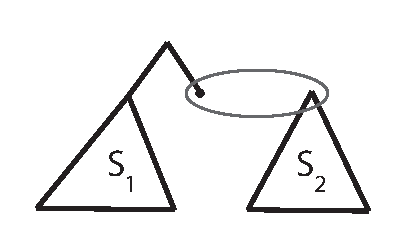
\includegraphics{pics/splay-join2}
\caption{JOIN2 pro splay stromy}
\label{splay-join2}
\end{figure}


\subsection{Algoritmus JOIN3}

Viz algoritmus \ref{alg:splay.join3}

\begin{algorithm}[!htb]
\caption{JOIN3($T_1$, x, $T_2$)}
\label{alg:splay.join3}
\begin{algorithmic}
\STATE vytvoříme vrchol $t$ reprezentující $x$
\STATE kořen $T_1$ je levý syn $t$ \\
\STATE kořen $T_2$ je pravý syn $t$
\end{algorithmic}
\end{algorithm}

Vytvoříme nový vrchol reprezentující $x$ a jeho synové budou $T_1$ -- levý,
$T_2$ -- pravý.

\begin{figure}[!htb]
\centering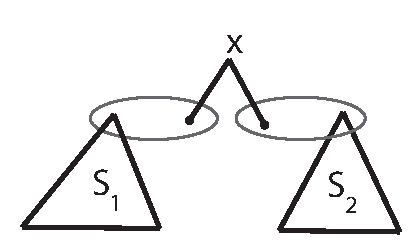
\includegraphics{pics/splay-join3}
\caption{JOIN3 pro splay stromy}
\label{splay-join3}
\end{figure}

\subsection{Algoritmus SPLIT}

Viz algoritmus \ref{alg:splay.split}

\begin{algorithm}[!htb]
\caption{SPLIT($x$,$T$)}
\label{alg:splay.split}
\begin{algorithmic}
%\STATE SPLAY(x)
%\IF {kořen T reprezentuje x}
%  \STATE $T_1$ podstrom levého syna kořene
%       \STATE $T_2$ podstrom pravého syna kořene
%       \STATE výstup $T_1$, $T_2$, x, $x \in S$
%  \ELSE
%       \IF {kořen T reprezentuje prvek $<$ x}
%          \STATE $T_2$ podstrom pravého syna kořene T
%	       \STATE $T_1 = T - T_2$
%	  \STATE T1 podstrom pravého syna kořene T
%	       \STATE $T_2 = T - T_1$
%       \ENDIF
%       \STATE výstup $T_1$, $T_2$, $x \in S$
%\ENDIF
\STATE SPLAY($x$)
\STATE $y$ = prvek reprezentovaný kořenem
\STATE $T_1$ = podstrom levého syna kořene
\STATE $T_2$ = podstrom pravého syna kořene
\IF {$y = x$}
  \STATE výstup $T_1$, $T_2$
  \STATE $x \in T$
\ELSIF {$y < x$}
  \STATE výstup $T \setminus T_2, T_2$
\ELSE
  \STATE výstup $T_1, T \setminus T_1$
\ENDIF
\STATE $x \not\in T$
\end{algorithmic}
\end{algorithm}

\mnote{zde chybi obrazek, ale celkem není pro pochopení potřeba :)}


\subsection{Algoritmus DELETE}

Mechanismus rušení uzlu (splay delete) je poněkud složitější. Uzel, 
který se má zrušit, se mechanismem splay přesune na pozici kořene. 
Zrušením kořene získáme 2 podstromy. Mechanismus splay se dále aplikuje 
na bezprostředního předchůdce a není-li tak následníka zrušeného uzlu 
(ve smyslu relace uspořádání - v průchodu inorder). Tím se tento uzel 
dostane do pozice kořene levého podstromu. Podle pravidel vyhledávacího 
stromu musí být všechny uzly levého podstromu menší než jeho kořen a 
všechny uzly pravého podstromu větší. Proto musí mít levý podstrom kořen 
vpravo volný a na toto místo se připojí pravý podstrom. Tento postup má 
symetrickou - levou versi. Operace "Splay Delete", rušící uzel D XXX je 
uvedena na obr.2.2. XXX
\par
Viz algoritmus \ref{alg:splay.delete}

\begin{algorithm}[!htb]
\caption{DELETE(x)}
\label{alg:splay.delete}
\begin{algorithmic}
\STATE SPLAY(x)
\IF {kořen reprezentuje x}
  \STATE $T_1$ je podstrom levého syna kořene T
       \STATE $T_2$ je podstrom pravého syna kořene T
       \STATE T $\leftarrow$ JOIN2($T_1$, $T_2$)
\ENDIF
\end{algorithmic}
\end{algorithm}

jiný zápis:
\begin{algorithmic}
\STATE $T_1, T_2 \leftarrow SPLIT(x, T)$
\STATE $T \leftarrow JOIN2(T_1, x, T_2)$
\end{algorithmic}

\subsection{Algoritmus INSERT}

Mechanismus vkládání (splay insert) vloží uzel jako list stejným 
způsobem jako BVS, ale potom se aplikuje na vložený uzel mechanismus 
"splay", který opět posune vložený uzel na pozici kořene. Operace
"Splay 
insert" uzlu s klíčem C XXX je uvedena na obr. \ref{splay-insert}.
\par


\begin{figure}[!htb]
\centering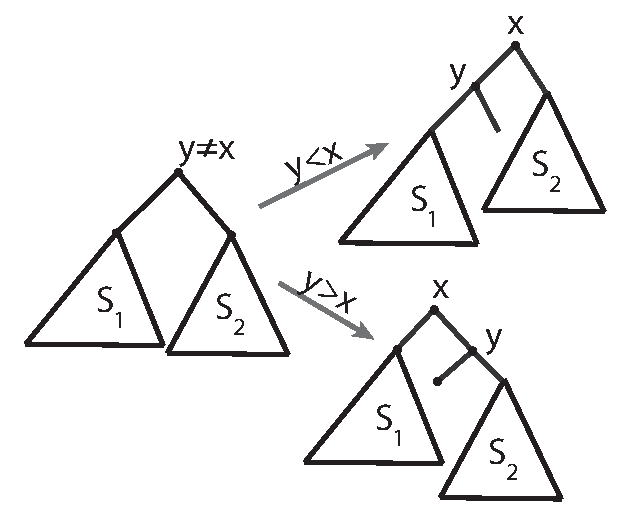
\includegraphics{pics/splay-insert}
\caption{INSERT(x) pro splay stromy}
\label{splay-insert}
\end{figure}


Viz algoritmus \ref{alg:splay.insert}

\begin{algorithm}[!htb]
\caption{INSERT(x)}
\label{alg:splay.insert}
\begin{algorithmic}
\STATE SPLAY(x)
\IF {kořen nereprezentuje x}
  \IF {kořen stromu reprez. prvek $<$ x}
          \STATE $T_2$ je podstrom pravého syna kořene
               \STATE $T_1$ = T - $T_2$ 
	  \ELSE 
	       \STATE T1 je podstrom levého syna kořene
	       \STATE $T_2$ = T - $T_1$
       \ENDIF
       \STATE JOIN3($T_1$, x, $T_2$)
\ENDIF
\end{algorithmic}
\end{algorithm}

jiný zápis:
\begin{algorithmic}
\STATE $T_1, T_2 \leftarrow SPLIT(x, T)$
\STATE $T \leftarrow JOIN3(T_1, x, T_2)$
\end{algorithmic}

\subsection{Algoritmus CHANGEWEIGHT}

Viz algoritmus \ref{alg:splay.chgw}

\begin{algorithm}[!htb]
\caption{CHANGEWEIGHT(x, $\triangle$)}
\label{alg:splay.chgw}

\begin{algorithmic}
\STATE SPLAY(x)
\IF {x je reprezentován v kořeni}
	\STATE k váze x přičti $\triangle$
\ENDIF
\end{algorithmic}
\end{algorithm}

Předpokládejme, že $w(x)$ je váha prvku a je to kladné celé číslo.
\par
$tw(x)$ - totální váha $x$, je to součet vah všech prvků v podstromě
určeném $x$.

\begin{priklad}
\mnote{chybí obrázek, tady je to nejake zmatene}
% XXX obr

$tw(a) = w(a) + w(b) + w(c)$ \\

$r(x)$ je $rank(x)$ \\
$r(x) = \lfloor \log tw(x) \rfloor$

$bal(konfigurace) = \sum \{ r(x) : x \in konfigurace \}$

Pro strom $T$ je $tw(x) = tw(\text{kořen }T)$ \\
	       $r(T) = r(\text{kořen }T)$
\end{priklad}

\begin{lemma}
Nechť $T$ je binární vyhledávací strom, $t$ je vnitřní vrchol a $u$,$v$ jsou
synové $t$. Pak $r(t) > min\{r(u), r(v)\} (r(list) = -\infty)$.
\end{lemma}

\begin{proof}
Předpokládejme, že $tw(u) \leq tw(v)$\\
$$
r(t) = \lfloor \log tw(t) \rfloor \geq \lfloor \log 2tw(u) \rfloor =
1 + \lfloor \log tw(u) \rfloor = 1 + r(u)
$$
\end{proof}

\subsection{Algoritmus SPLAY}

Volání algoritmu SPLAY se většinou zapisuje jako SPLAY($x$), kde explitictně
neuvádíme strom, na kterém je operace prováděna - to většinou vyplyne z
kontextu. Tam, kde je nutné uvést, na kterém stromě se operace SPLAY
provádí (např. v implementaci operace JOIN2, píšeme volání jako 
SPLAY($x$,$T$).

Viz algoritmus \ref{alg:splay.spl}

\begin{algorithm}[!htb]
\caption{SPLAY(x)}
\label{alg:splay.spl}
\begin{algorithmic}
\STATE SPLAY(x)
\STATE $t$ $\leftarrow$ kořen
\WHILE {$t$ není list a $t$ nereprezentuje $x$}
	\IF {$x < t$}
		\STATE $t$ $\leftarrow$ levý syn $t$
	\ELSE
		\STATE $t$ $\leftarrow$ pravý syn $t$
	\ENDIF
\ENDWHILE
\IF {$t$ je list}
	\STATE $t \leftarrow otec(t)$
\ENDIF
\WHILE {$t$ není kořen}
	\IF {$otec(t)$ je kořen}
	  \STATE rotace($t$, otec($t$))
	\ELSE
		\IF {otec($t$) i $t$ jsou oba leví (praví) synové}
		  \STATE rotace(otec($t$), děd($t$))
		  \STATE rotace($t$, otec($t$))
		\ELSE
		  \STATE dvojitá rotace($t$, otec($t$), děd($t$))
		\ENDIF
	\ENDIF
\ENDWHILE
\end{algorithmic}
\end{algorithm}

V algoritmu
SPLAY (algoritmus \ref{alg:splay.spl}) se používá jednoduché 
(obr. \ref{splay-rot}) a dvojité (obr. \ref{splay-dvojrot}) rotace.
Vrchol $t$ se po skončení operace SPLAY(x) dostane do kořene. Toho
dosáhneme tak, že v prvním cyklu najdeme vrchol $t$ reprezentující prvek
$x$, v druhém cyklu přesouváme vrchol $t$ do kořene.

\begin{figure}[!htb]
\centering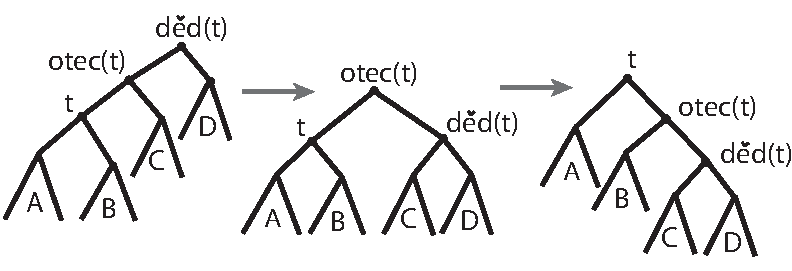
\includegraphics{pics/splay-rot}
\caption{Dvakrát jednoduchá rotace pro SPLAY($x$)}
\label{splay-rot}
\end{figure}

\begin{figure}[!htb]
\centering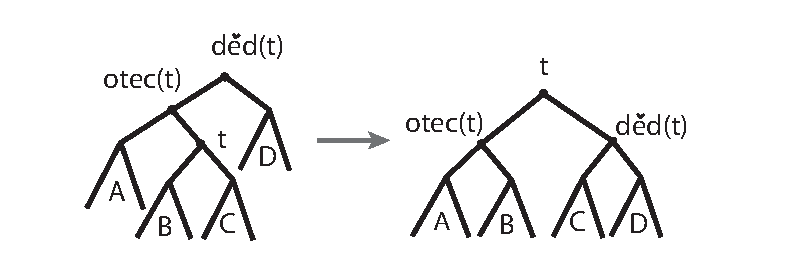
\includegraphics{pics/splay-dvojrot}
\caption{Dvojrotace pro SPLAY($x$)}
\label{splay-dvojrot}
\end{figure}


\subsection{Amortizovaná složitost SPLAY}

Budeme předpokládat, že $v(x) \geq 1$ pro každé $x$. \\
Totální váha $x = w(x)$, což je součet vah všech prvků v podstromu vrcholu
reprezentujícího $x$.
\par
Značíme $r(x) = \lfloor log_2 w(x)\rfloor = \text{rank vrcholu } x$
\par
Pro strom $T$: \\
$$w(T) = w(\text{kořen}(T)) \\
r(T) = r(\text{kořen}(T))$$
\par
bal(konfigurace) = součet ranků všech vrcholů v množinách tvořících
konfigurace
\par
Náš cíl : Budeme chtít ukázat, že amortizovaná složitost operací je
$O(\log\frac{w(T)}{v(x)})$, když $T$ reprezentuje $S$.
\par
Čas operace SPLAY = počet běhů druhého cyklu, který vrchol $t$ 
transportuje do kořene.


\begin{lemma}
\label{splay-pomlemma}
Pomocné lemma: Mějme vrchol $w$ ve stromě $T$ se syny $y_1$ a $y_2$ a
předpokládejme, že $y_1$, $y_2$ nejsou listy. Když $w$ reprezentuje $a$,
$y_r$ reprezentuje $b_i$ pro $i=1,2$, pak $rank(a) > min\{r(b_1),r(b_2)\}$
\end{lemma}

\begin{proof}
\begin{figure}[!htb]
\centering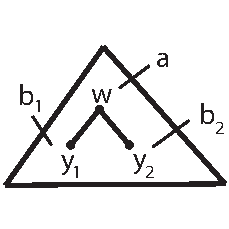
\includegraphics{pics/splay-lemma}
\caption{Pro důkaz pomocného lemmatu pro splay stromy}
\label{splay-lemma}
\end{figure}

Situaci lze vidět na obrázku \ref{splay-lemma}. 
\par
Zřejmě $r(a) \geq r(b_1)$ a $r(a) \geq r(b_2)$, tedy $r(b_1) \neq r(b_2) 
\Rightarrow r(a) > min\{r(b_1),r(b_2)\}$
\par
\begin{equation}
\begin{split}
r(a) 
& = \lfloor \log_2 w(a) \rfloor \geq \lfloor (w(b_1) + w(b_2)) \rfloor \\
& \geq \lfloor \log_2(2 - min\{w(b_1),w(b_2)\}) \\
& = 1 + \log_2 min\{w(b_1),w(b_2)\} \\
& = 1 + min\{w(b_1),w(b_2)\}
\end{split}
\end{equation}
\end{proof}

\begin{theorem}
Amortizovaná složitost operace SPLAY($x$,$T$) $\leq 3(r(T)-r(t)) + 1$, 
kde $t$ je vrchol, který transportujeme do kořene. $T$ je strom
reprezentující $S$.
(když $x$ je prvek reprez. množiny, pak $t$ reprezentuje $x$, jinak je to buď
největší nebo nejmenší prvek menší (větší) než $x$)
\end{theorem}

\begin{proof}
Označme $T_0$ původní strom, $T_i$ strom po $i$-tém běhu druhého cyklu 
v SPLAY a
předpokládejme, že druhý cyklus běží k-krát. (tj. $T_k$ je výsledný strom)
\par
Amortizovaná složitost (SPLAY($x$,$T$)) 
\mnote{$\text{``čas operace``} = k$}
\begin{equation}
\begin{split}
& = \text{čas operace} + bal(\text{výsledná konfigurace}) - 
bal(\text{původní konfigurace}) \\ 
& = k + bal(T_k) - bal(T_0) \\
& = \sum_{i=1}{k}(1 + bal(T_i) + bal(T_{i-1})
\end{split}
\end{equation}
\mnote{$balance = \sum \text{rank v }T_k$}

Označme $r_i$ rank ve stromě $T_i$, nechť $u_i$ je otec $t$ ve stromě
$T_i$ a když $u_i$ není kořen $T_i$, pak $v_i$ je otec $u_i$ v $T_i$.

\begin{itemize}
\item a)
$u_i$ je kořen: \\
chci odhadnout $1 + bal(T_i) - bal(T_{i-1})$ :
\begin{equation}
\begin{split}
& 1 + bal(T_i) - bal(T_{i-1}) \\
& = 1 + \sum_{z \text{ reprezentován v }T_i} r_i(z) + \sum_{z} r_{i-1}(z) \\
& = 1 + r_i(u_{i-1}) + r_i(t) - r_{i-1} - r_{i-1}(t) \\
& = 1 + r_i(u_{i-1}) - r_{i-1}(t) 
\leq 1 + 3(r_{i-1}(u_{i-1}) - r_{i-1}(t))
\end{split}
\end{equation}

\begin{figure}[!htb]
\centering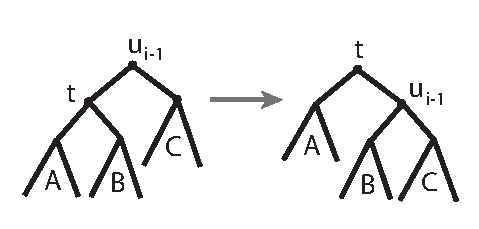
\includegraphics{pics/splay-amortproof1}
\caption{Pro důkaz amort. složitosti operace SPLAY}
\label{splay-amortproof1}
\end{figure}

Platí $r_i(t) = r_{i-1}(u_{i-1})$, protože stromy $A$,$B$,$C$ na obr.
\ref{splay-amortproof1} jsou stejné.
\par
Platí
$$
r_i(u_{i-1}) \leq r_{i-1}(u_{i-1}) 
$$
$$
r_{i-1}(u_{i-1}) \geq r_{i-1}(t)
$$

\item b)
  $u_{i-1}$ není kořen: 
  \begin{enumerate}
  \item $u_{i-1}$ je jiný syn v $T_{i-1}$ než $t$
  \item $u_{i-1}$ je stejný syn v $T_{i-1}$ jako $t$
  \end{enumerate}
\end{itemize}

\par
\begin{itemize}
\item ad b1) : \\
\begin{equation}
\begin{split}
& 1 + bal(T_i) - bal(T_{i-1} = \sum_{z}{} r_i(z) - \sum_{z}{} r_{i-1}(z) \\
& = 1 + r_i(t) - r_i(u_{i-1}) + r_i(v_{i-1}) - r_{i-1}(t) - r_i(u_{i-1}) -
	r_{i-1}(v_{i-1}) \\
& = 1 + r_i(u_{i-1}) + r_i(v_{i-1}) - r_{i-1}(t) - r_{i-1}(u_{i-1}) \\
& \leq 2(r_{i-1}(v_{i-1}) - r_{i-1}(t)) \\
& \leq 3(r_{i-1}(v_{i-1}) - r_{i-1}(t))
\end{split}
\end{equation}

První nerovnost v odvození platí, protože 
$1 + r_i(u_{i-1}) + r_i(v_{i-1}) = 2r_{i-1}(t) = 2r_{i-1}(v_{i-1})$.
\par
Amortizovaná složitost během cyklu: $\leq 3(r_i(v_{i-1}) - r_{i-1}(t))$

\item ad b2) : \\

$1 + bal(T_i) - bal(T_{i-1}) = ... 
= 1 + r_i(u_{i-1}) + r_i(v_{i-1}) - _{i-1}(t) - r_{i-1}(u_{i-1}) \leq$

  \begin{itemize}
  \item{$\alpha$} \\
    Předpoklad: $r_{i-1}(t) < r_i(v_{i-1})$ \\
    Pak platí: \\
    $\leq 1 + 2(r_{i-1}(v_{i-1}) - r_{i-1}(t)) 
    \leq 3(r_i(v_{i-1}) - r_{i-1}(t))$
  \item{$\beta$} \\
    Předpoklad: $r_{i-1}(t) = r_i(v_{i-1})$, $r_i(t) > r_i(v_{i-1})$ \\
    $... = 1 + r_i(u_{i-1}) + r_i(v_{i-1}) - r_{i-1}(t) - r_{i-1}(u_{i-1})
    \leq 2(2(r_{i-1}(v_{i-1}) - r_{i-1}(t))
    \leq 3(r_i(v_{i-1}) - r_{i-1}(t))$
  \item{$\gamma$} \\
    Předpoklad: $r_i(t) = r_i(v_{i-1}) - r_{i-1}(v_{i-1}) = r_{i-1}(t)$ \\
    Vím: $r_{i-1}(t) = r'(t) = r_{i-1}(v_{i-1}) = r'(u_{i-1}) 
    = r_i(t) = r_i(v_{i-1}) = r'(v_{i-1})$
    spor s lemmatem \ref{splay-pomlemma}.
    $\Rightarrow$ případ $\gamma$ nemůže nastat
  \end{itemize}

  Závěr pro b) : Amortizovaná složitost během cyklu 
  $\leq 3(r_i(v_{i-1}) - r_{i-1}(t))$

\end{itemize}

Vždy platí $r_i(v_{i-1}) = r_i(t)$ \\
\begin{equation}
\begin{split}
& \sum_{i=1}{k}(1 + bal(T_i) - bal(T_{i-1})) \\
& \leq \sum_{i=1}{k} 3(r_i(v_{i-1}) - r_{i-1}(t)) \\
& = 1 + 3(r_{k-1}(v_{k-1}) - r_0(t)) = 1 + 3(r_o(T) - r_0(t))
\end{split}
\end{equation}


%
% XXX toto je puvodni dukaz jsem napsal nekdy v 2003:
%
%rozdělíme podle akce, která se provádí ve while cyklu
%\begin{itemize}
%\item while cyklus provádí rotace
%
%$= 1 + r'(u) - r(v) \leq 1 + r(u) + r(v)$ \\
%$\leq 1 + 3(r(u) - r(v))$
%
%protože $x$ má v původním i novém stromě stejné prvky
%\mnote{nečitelné}
%$r(u) = r'(t)$ \\
%$r'(u) \leq r'() = r(u)$
%
%\par
%% b)
%\item while cyklus provádí dvojitou rotaci
%
%\mnote{tady chybi obr.}
%
%\begin{multline}
%\label{amort-dvojrotace}
%\text{Amortizovaná složitost této operace} \\
%\text{= čas operace + bal(nová konf.) - bal(původní konf.) =} \\
%= 1 + r'(u) - r(v) - r(u) - r(t)
%\end{multline}
%
%pro $x \neq t,u,v$ platí $r(x) = r'(x)$ \\
%$r(v) = r'(t)$
%
%\begin{itemize}
%  \item
%  \begin{multline}
%  r(v) > r(t), pak r'(u),r'(v) \leq r'(t) = r(v)\\
%  r(u) \geq r(t), 1 \leq r(v) - r(t) \stackrel{\text{ \ref{amort-dvojrotace}
%  }}{\leq} \\
%  r(v) - r(t) + 2r(u) - 2r(t) = 3(r(v) - r(t))
%  \end{multline}
%  
%  \item
%  r(v) = r(t), pak podle lemmatu $r'(t) > min\{r'(u), r'(v)\}$ plati \\
%  \begin{multline}
%  2r'(t) \geq r'(u) + r'(v) + 1 
%    \stackrel{\text{ \ref{amort-dvojrotace} }}{\leq} \\
%  2r(u) - 2(r(t) = 2(r(v) - r(t)) = (r(t) = 0) 3(r(u) - 3r(t))
%  \end{multline}
%  
%\end{itemize}
%\end{itemize}

\end{proof}




% -------------------------------------------------------------------------

\subsection{Amortizovaná složitost ostatních operací}

\begin{defn}
Amortizovaná složitost operace $SPLAY(x,T) \leq 1 + 3(r(T)-r(t))$, kde $t$
je prvek, který se přemístí do kořene.
\end{defn}

\par
Označme $t_{-}$ prvek ve stromě T, který reprezentuje největší prvek 
$\leq x$.
\par
Označme $t_{+}$ prvek ve stromě T, který reprezentuje nejmenší prvek 
$\geq x$.
\par
Když $x$ je reprezentováno $T$, pak $t_{-} - t_{+}$ je prvek reprezentující
$x$.
\par
Jednotlivé operace mají následující amortizované složitosti:

\begin{itemize}
\item $SPLAY(x,T) = O(\log\frac{w(T)}{min\{w(t_{-}),w(t_{+})\}})$ \\
\item $MEMBER(x,T) = O(\log\frac{w(T)}{min\{w(t_{-}),w(t_{+})\}})$ \\
\item $SPLIT(x,T) = O(\log\frac{w(T)}{min\{w(t_{-}),w(t_{+})\}})$ \\
\item $CHANGEWEIGHT(x, \triangle) = O(\log\frac{
w(T) - max\{\triangle,0\}}{min\{w(t_{-}),w(t_{+})\}
})$ \\
\item $JOIN3(T_1, x, T_2) = O(\log\frac{w(T_1)+w(T_2)+v(x)}{v(x)})$
\end{itemize}

Označme $t_{\infty}$ prvek v $T_1$, který reprezentuje největší prvek z
$T_1$. Pak amortizované složitosti pro zbývající operace jsou
následujicí:
\par

\begin{itemize}
\item $JOIN2(T_1,T_2) = O(\log\frac{w(T_1) + w(T_2)}{w(t_{\infty})})$ \\
\item $DELETE(x,T) = O(\log\frac{w(T)}{min\{w(t_{-}),w(t_{+}),w(t_{1}\}})$ \\
\end{itemize}

Prvek $t_1$ je prvek $T_1$, který reprezentuje v $T$ největší prvek $\leq x$.

\begin{itemize}
\item $INSERT(x,T) = O(\log\frac{w(T) + v(x)}{min\{w(t_{-}),w(t_{+})\}})$
\end{itemize}

% priklad pro SPLAY stromy ----------------------------------------------

\begin{priklad}
Mějme množinu $X={x_1,...,x_n}$ a pravděpodobnosti pro výskyt operace
MEMBER(x). Nechť $U$ je optimální binární vyhledávací strom. Nechť $T$ je
binární vyhledávací strom reprezentující $X$. $P$ je posloupnost operací
MEMBER(x) vyhovující daným pravděpodobnostem.
\par
Chceme aplikovat $P$ na strom $T$, kde pro implementaci použijeme strategii
SPLAY stromů.
\par
Srovnáme čas, který tato strategie vyžaduje s časem obvyklé implementace
MEMBER při aplikaci $P$ na $U$.
\par
Definujeme $v(x) = 3^{d-d(x)}$, kde d je hloubka stromu $U$ a $d(x)$ je
hloubka prvku v $U$ reprezentujícího prvek $x$.
\par
Spočítáme totální váhu prvku $x$:
$$w(x) = \sum_{i=0}{d-d(x)} 2^i3^{d-d(x)-i} 
\leq 3^{d-d(x)} \sum_{i=0}{d-d(x)} (\frac{2}{3})^i \leq 3^{d-d(x)+1}$$
\par
Pak platí: \\
$r(x) \leq d-d(x)+1$ \\
$r(T) \leq d+1$, (prvek v kořeni má hloubku $0$)
\par
Amortizovaná složitost operace MEMBER(x) 
$$\leq O(d(x)) = 
O(r(T)-r(x)) = O(d+1-d+d(x)-1) = O(d(x))$$
\par
Čas posloupnosti $P$ použité na strom $T$ a implementované strategií SPLAY 
$$= (\sum_{\text{operace v P}}{} \text{amortizovaná složitost operací v P}) +
bal(T) = O(\text{čas P pro strom U} + bal(T))$$
\par
$bal(T)$ je balance stromu $T$. 
$$bal(T) = \sum_{x \in X}{} r(x) = 
\sum_{x \in X}{} d+1 = O(x^2)$$
\par
$$\Rightarrow  O(\text{čas P pro strom U}) + bal(T) = 
O(\text{čas P pro U} + x^2)$$
\mnote{tady bylo ve vzorci něco jako $|x^2|$ (?)}
\par
Závěr: pro dlouhé posloupnosti snad téměř stejné jako opt. BVS.
\end{priklad}

% EOF
